\section{Measurement and Data}\label{sec:method}

We now describe the data that each ISP provides concerning the
utilization of each network port, and how this data is sampled and
aggregated.  

Sampling and aggregation can affect the accuracy of the
resulting measurements, and we discuss the effects of sampling and
aggregation later in this section.  In addition to discussing the
methods that the ISPs use, we also describe alternative approaches to
measuring network utilization and the advantages and drawbacks of each
method.


\subsection{Traffic Flow Statistics and Utilization}
A common method for gathering statistics about the utilization of a
network---and the method that this project uses---is to gather what are
often referred to as ``flow statistics''; the most common version of
flow statistics is likely the IPFIX protocol (often instantiated in
Cisco products as ``NetFlow'')~\cite{rfc7011}.  Many other vendors have conformed to a
similar standard when exporting records about traffic flows.

A IPFIX record contains metadata about the flow, including the number
of bytes transferred, the number of packets in the flow, the start and
end times for the flow, and the network interface associated with the
flow.  Accordingly, the statistics in a flow record can give useful
information about the average utilization over a period of time in terms
of either bytes or packets.  For example, if the flow record has a
duration of ten seconds and reports that 1 gigabyte of traffic was
transferred during that ten seconds, then the average utilization over
that ten-second period would be 800 megabits per second (eight gigabits
per ten seconds).  The flow statistics can also be used to compute
average packet rates, in terms of packets per second, in a similar
manner. 


\begin{figure}[t]
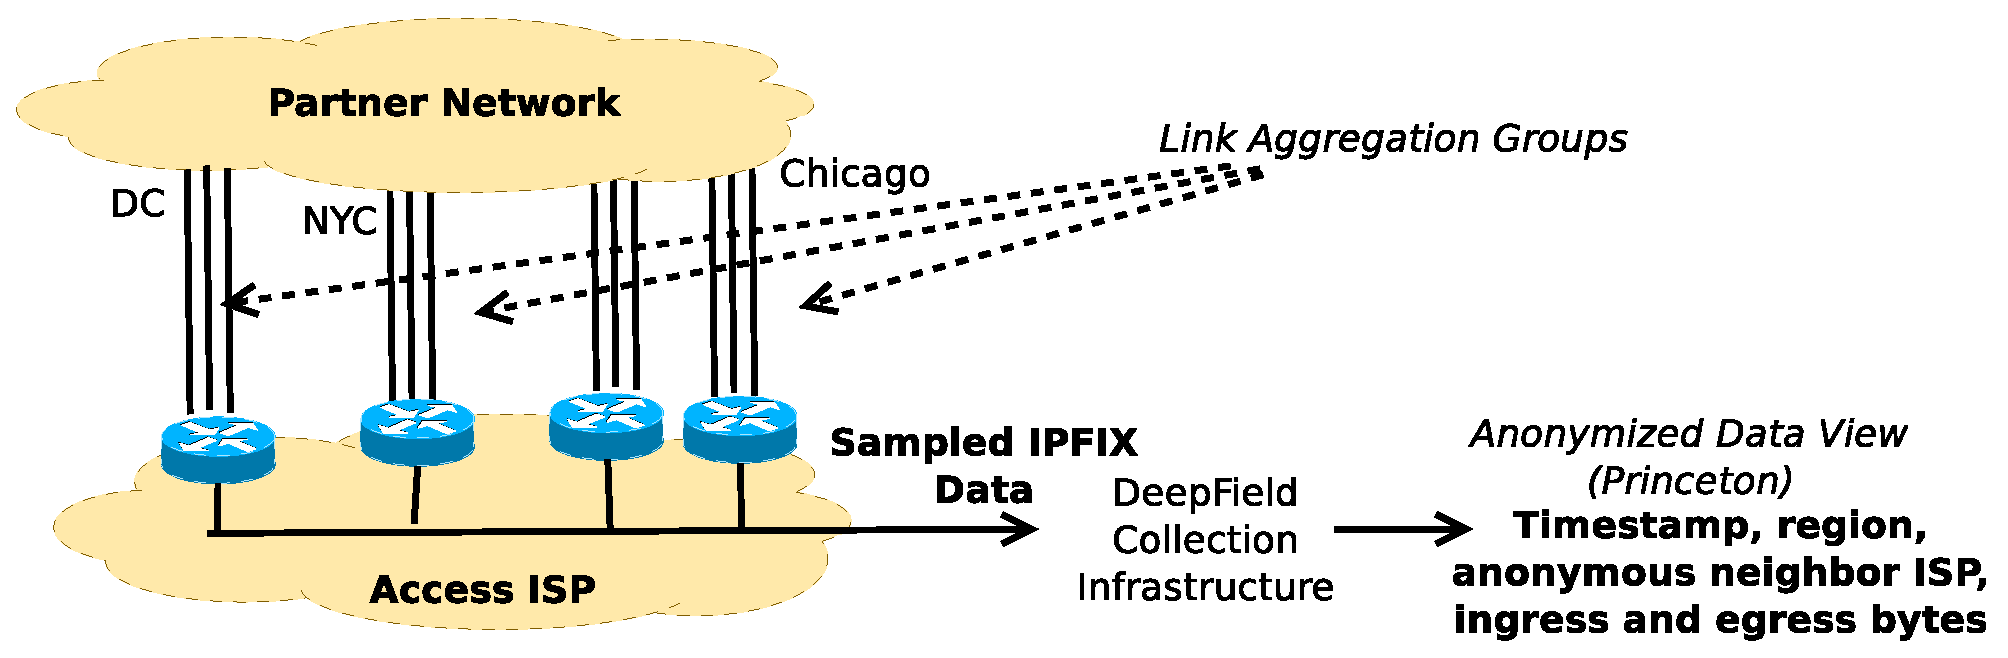
\includegraphics[width=\linewidth]{arch2}
\caption{Data collection
  infrastructure and approach.} 
\label{fig:arch}
\end{figure}

The traffic in this dataset covers interconnection points
for access ISPs that account for about 50\% of the broadband subscribers in the United
States. 
Figure~\ref{fig:arch} shows how data is collected from each
interconnection point between an access ISP and neighboring partner network.  Each participating access
ISP may connect to a partner network in multiple geographic regions. The
access ISP collects IPFIX data at each interface that interconnects with
a neighboring partner network.
The traffic statistics that each ISP reports are based on IPFIX records
that are exported at least as frequently as every 60 seconds and subsequently
aggregated across a 
link group; to protect the confidentiality of information pertaining to
usage on specific interconnects, the data is aggregated into a single link group per geographic
region. (Section~\ref{sec:aggregation} describes this approach in more
detail, and how it affects the conclusions we can draw.) The statistics
represent an aggregate that is computed based on 
the sum of peak five-minute intervals in each hour, for each {neighbor
  network, circuit group} pair.

The dataset contains about 97\% of links from all participating ISPs in
any given month; the only links that are missing from the data set are
links that are not configured in DeepField's measurement system.  All
interconnections between participating ISPs and neighboring partner
networks are private (i.e., none of the interconnections in this study
involve public IXP switch fabrics).  Each row in the dataset that CITP
receives includes the following statistics:
\begin{itemize}
\itemsep=-1pt
\item	Timestamp (representing a five-minute interval)
\item	Region (representing an aggregated link group)
\item	Anonymized partner network
\item       Access ISP
\item	Total ingress bytes
\item	Total egress bytes
\item       Capacity
\end{itemize}
\noindent
Because flows do not begin and end on discrete five-minute intervals,
each five-minute timestamp represents the sum of utilization of active
traffic flows that were active during that interval. Suppose that, at a
given time, a set of flows are active. Then, the total ingress bytes for
that five-minute interval for a single flow would be the average bitrate
for that flow over its total duration, multiplied by the amount of time
that the flow was active during the given five minute interval. The
total utilization for the link aggregation group is the sum of all such
statistics, for any flows that were active during that five-minute
interval. 


\subsection{Aggregation and Load Balancing}\label{sec:aggregation}
When measuring the contribution of a traffic flow to a link's utilization,
it is also important to ensure that flows are not double counted. An
ISP's ports may be configured as a link aggregation group (we are aware
of this configuration for at least one ISP in the study).  In this ISP's case,
the router balances outbound traffic flows across the links; a single
flow always goes across a single link. The allocation of outbound
traffic flows to links is based on a hashing algorithm on the router;
given enough traffic flows, this type of load balancing typically works
well enough to balance load evenly across the available links in any
given aggregation group.  It is extremely rare for any ISP
to have multiple LAGs in a region to a given partner network.

We are cognizant of only the outbound load balance mechanisms for all of
the ISPs that contribute data; we are unaware of the traffic load
balance practices of partner networks that do not participate in the study, but, for
the purposes of assessing inbound traffic loads across links in an
aggregation group, it is likely reasonable to assume that these ISPs
also use typical load balancing practices for outbound traffic (and,
hence, we can assume a relatively uniform load balance of inbound
traffic flows for a link aggregation group). 

In networks where there exist only a small number of flows, such as in
commercial VPNs, it is possible that utilization across links might
become unbalanced, but on links carrying consumer traffic, such as those
in this study, it would be highly unusual for traffic to be unevenly
balanced across links, due to the nature of the router hashing function,
which is designed to randomly assign these flows to available links.
Thus, although traffic statistics are reported in aggregate across an
aggregation group, it is highly unlikely that we would encounter a
situation where average traffic flow statistics would report low
congestion, but some links in the aggregation group would be congested
while others would be underutilized. 

\subsection{Sampling}


IPFIX records must be sampled, meaning that the statistics in any given
record are based not on all of the packets in that flow, but rather a
random sample of the packets in that flow. In this project, ISPs report
statistics that are based on sampled IPFIX records.  Typically, IPFIX
sampling can take one of two forms: {\em random} and {\em
  deterministic}. If the sampling factor is N, then random sampling will
incorporate the statistics for any given packet with probability 1/N; on
the other hand, deterministic sampling will incorporate the statistics
based on every Nth packet deterministically.

The effects of sampling on overall traffic volume estimation bears some
discussion. Certainly, when trying to estimate certain characteristics,
such as the number of small flows that cross an interface, or the
overall distribution of flow-sizes, aggressive sampling can distort
measurement accuracy. On the other hand, estimating overall utilization
is possible in general---flows may be missed entirely, but on
average, some fraction of the small flows will be captured. Attempts to
normalize the flow sizes for small flows will result in inaccurate
estimates of the flow sizes of these small flows, but the estimates for
overall traffic volume should remain reasonably accurate. For example,
suppose that a link creates flow statistics based on a packet-sampling
rate of 1/1,000. In the extreme case, suppose that each flow is a single
packet. Then, on average, the statistics will reflect one in every
thousand flows, and attempts to normalize these statistics would result
in an estimate of one flow of 1,000 packets. Clearly, the flow-size
estimates are incorrect, but the total utilization is accurate,
on average.   

% IPFIX sampling can make flow size estimation difficult
% because small flows can be missed entirely (e.g., if no packets are
% incorporated into the statistics, there may be no flow table entry at
% all). Additionally, if a packet is sampled from a small flow, then
% multiplying by N is typically sufficient to recover or approximate the
% size of the resulting flows.  

%This effect woud be problematic if we were concerned in
% estimating the presence of small flows or computing flow-size
% distributions. However, since we are concerned only with aggregate
% utilization for this study, the sampling effects are less detrimental.

% If a traffic link were carrying a large number of small flows, many of
% the flows might not have corresponding traffic flow statistics at all.
% For example, suppose that a DNS flow is only one packet; if random
% sampling happens to generate an IPFIX record based on the packet, even
% if the sampling factor N is 1,000, then post hoc analysis will estimate
% the flow size as 1,000 packets, even though the actual number of packets
% in the flow is only one packet. Of course, sampling will only sample one
% in 1,000 one-packet flows, so if we have 1,000 one-packet flows, the
% resulting estimation of {\em aggregate} capacity will be unaffected: the
% estimate will reflect a single thousand-packet flow, as opposed to one
% thousand single-packet flows.  In these cases, the bytes contributed by
% these smaller traffic streams might not be accounted for at all, thereby
% causing an underestimation of link utilization. The extent to which this
% is the case on the interconnection links for these ISPs does deserve
% further investigation before it is possible to definitively say that the
% capacity estimation is accurate. We would need to know more about the
% number of traffic flows that have only a small number of packets. Given
% what we know about application traffic makeup on today's Internet,
% however, one would expect this contribution to be dwarfed by large,
% long-running video streams, given current traffic mixes, but more study
% of this issue is necessary.


The observation
that sampled IPFIX records are sufficient for aggregate capacity
utilization holds empirically, as well. We compared the SNMP byte
counters to sampled IPFIX records with a 1/8,000 sampling rate across
250 interconnect links for one of the largest participating ISPs in the
study for a single day. The mean and median of the ratio
between both metrics were both around 0.98, with a standard deviation of
0.095. As ISPs increase their sampling rates, the accuracy of IPFIX
relative to SNMP should improve further.

In conclusion, the average of sampled utilization across port groups may
underestimate utilization, and averaging across port groups may not be
able to characterize the distribution of utilization (and congestion)
across the group (e.g., some ports may be congested while others remain
uncongested). Yet, we can certainly use this data to determine with confidence
whether there exist uncongested ports in a region between a pair of
networks.


\paragraph{Sampling rates in this study.}
Most of the Internet service providers in the study report traffic flow
statistics based on a sampling rate of 1/1,000, meaning that statistics
are collected based on a sampling of every thousandth packet, on
average; all of the ISPs who are contributing data implement a sampling
rate of at least 1/8,000.  Some of the ISPs in the study use deterministic sampling
and others use random sampling; given that the goal is to estimate
capacity on links where much of the traffic flows that contribute to
congestion are large, long-running video streams---which have fairly
large packet and byte counts---neither the sampling rate nor the mode of
sampling should affect the accuracy in estimating the overall
utilization.

\subsection{Configuration and Topology}

Each participating Internet service provider (ISP) provides the
following information from configuration data, and from SNMP polling: 
\begin{itemize}
\item {\em Interconnection.} For each of an ISP's peers, the ISP's router
  configuration data provides information about which interface maps to
  each neighboring autonomous system (AS), as well as the policies
  associated with each connection, such as Border Gateway Protocol
  configuration options (e.g., local preference, and AS path
  prepending).  The router configuration also provides information such
  as the mapping of individual network interface names to the AS that
  the interface corresponds to. In this study, the next-hop AS was
  determined from BGP routing information gathered from the
  interconnection router. 

\item {\em Provisioning.} In addition to the mappings between interfaces and
  ASes that the configuration provides, SNMP polling data yields
  information about the interface capacity that is provisioned on each
  link.  
\end{itemize}

DeepField has the ability to collect this data from all routers in the
network---including those that peer directly with neighboring autonomous
systems (ASes) and those that are internal to the network. For the
purposes of this study, data from the border routers alone suffices, as
we are not concerned with internal utilization but rather only with
utilization that may occur at the edge of the network. 

\subsection{Public Use of Data}

Although the ISPs make the above data available to us, much of this data
is bound by mutual non-disclosure agreements between the ISPs and their
respective partner networks, due to the proprietary nature of
interconnections. As mentioned, both the existence and nature of any
particular interconnection is considered proprietary, as are the
decisions about where any particular ISP has a point of presence and
where any ISP tends to route different types of traffic.  These details
reflect both business strategy (e.g., provisioning), business
relationships, the source and destination of traffic demands, and
decisions about network management and operations.  We emphasize that
the restrictions on our ability to disclose data to the public result
not from a specific agreement with the ISPs but rather from the {\em
  mutual non-disclosure agreements between the ISPs and their content
  providers}, which are intended to protect both parties.

Due to the sensitive nature of much of this information, 
the public dataset reports utilization that is aggregated by region and
across at least three participating ISPs.
The
publicly released visualizations and underlying data include 
statistics about link aggregation groups, as we describe below.
The public dataset reports the following aggregate utilization statistics:
\begin{itemize}
\item For each ISP, across all interconnect links
  to all neighbor networks.
\item For each region, across all ISPs
\item Across all interconnects and all regions.
\item Across all links, both per-link and weighted by overall aggregate capacity.
\end{itemize}
\noindent
The public visualizations and underlying data, which we plan
to update monthly, reveal the following aggregate statistics and information: 
\begin{itemize}
\item Peak utilization at an interconnect, relative to total capacity, aggregated across ISPs in that region.
\item The fraction of interconnects that experience a percentage maximum
utilization, for the 95th percentile of five-minute intervals.
\item Utilization by region over time, for all regions with at least three operators.
\end{itemize}
\noindent
This level of aggregation does not make it possible to assess the
overall utilization of a particular ISP's connections to a neighboring
network, and analysis of the public data cannot show that there are no
highly utilized links. Although the private data has information about
utilization of individual interconnections, we are not permitted to
disclose statistics at this granularity; in an effort to disclose as
much information as possible, we have released certain information about
utilization of individual interconnection links, including the
distribution of utilization across these links.

 Demonstrating this result would require analysis of much more
fine-grained data.  Nonetheless, the public aggregate statistics
do provide evidence that each participating ISP and region has spare
capacity at respective interconnection points, as we discuss in more
detail in the coming sections.